\subsection{Graphs}\label{subsec:graphs}

\begin{example}\label{ex:konigsberg_bridges}
  A puzzle problem regarding the seven K\"onigsberg bridges was solved by Leonhard Euler in 1735 and published six years later as \cite{Euler1741}. In the English translation of the paper by \incite[ch. 1A]{BiggsLloydWilson1986}, the puzzle is described as follows in \S 2:
  \begin{displayquote}
    The problem, which I am told is widely known, is as follows: in K\"onigsberg in Prussia, there is an island \( A \). called the Kneiphof; the river which surrounds it is divided into two branches, as can be seen from \cref{fig:ex:konigsberg_bridges/schematic/drawing}, and these branches are crossed by seven bridges, \( a \), \( b \), \( c \), \( d \), \( e \), \( f \) and \( g \). Concerning these bridges, it was asked whether anyone could arrange a route in such a way that he would cross each bridge once and only once. I was told that some people asserted that this was impossible, while others were in doubt; but nobody would actually assert that it could be done. From this, I have formulated the general problem: whatever be the arrangement and division of the river into branches, and however many bridges there be, can one find out whether or not it is possible to cross each bridge exactly once?
  \end{displayquote}

  \begin{figure}[ht!]
    \frame{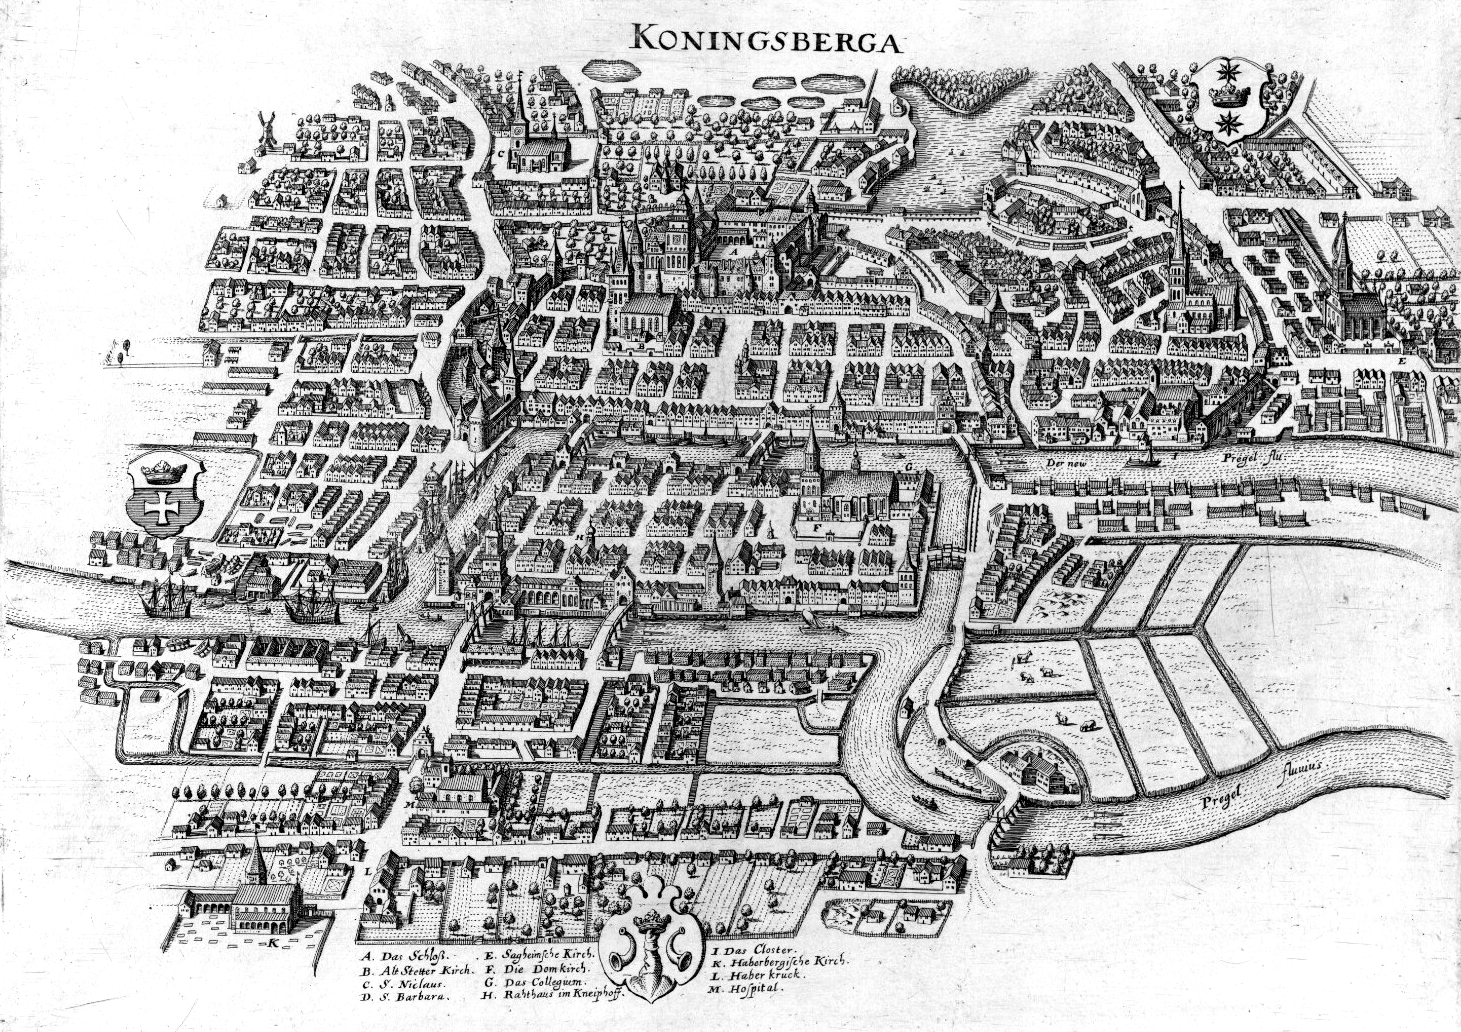
\includegraphics[width=\textwidth]{images/ex__konigsberg_bridges__illustration}}
    \caption{An illustration of K\"onigsberg by Matth\"aus Merian published in 1652 in \cite{MerianKönigsbergBridges}.}
    \label{fig:ex:konigsberg_bridges/illustration}
  \end{figure}

  This is considered to be the first paper in graph theory\fnote{The early history of graph theory can be found in \cite{BiggsLloydWilson1986}}. In \S 1 of his paper, Euler himself hints at the geometric nature of the problem\fnote{Topology did not exist at the time, so the problem could not have possibly been considered topological.}:
  \begin{displayquote}
    In addition to that branch of geometry which is concerned with magnitudes, and which has always received the greatest attention, there is another branch, previously almost unknown, which Leibniz first mentioned, calling it the geometry of position. This branch is concerned only with the determination of position and its properties; it does not involve measurements, nor calculations made with them. It has not yet been satisfactorily determined what kind of problems are relevant to this geometry of position, or what methods should be used in solving them. Hence, when a problem was recently mentioned, which seemed geometrical but was so constructed that it did not require the measurement of distances, nor did calculation help at all, I had no doubt that it was concerned with the geometry of position — especially as its solution involved only position, and no calculation was of any use. I have therefore decided to give here the method which I have found for solving this kind of problem, as an example of the geometry of position.
  \end{displayquote}

  To solve the puzzle, Euler denotes four pieces of land by \( A \), \( B \), \( C \) and \( D \) and considers sequences of adjacent pieces of land. This corresponds roughly to some modern definitions for both \enquote{walk} and \enquote{path} --- see the discussions in \fullref{rem:graph_walk_terminology}. Later, in \S 15, he even considers alternating sequences of pieces of land and bridges, which exactly corresponds to finite walks as defined in \fullref{def:graph_walk}. We will formalize the requirement of crossing each bridge exactly once by introducing Eulerian walks in \fullref{def:eulerian_walk}.

  \begin{figure}[ht!]
    \begin{subcaptionblock}{0.55\textwidth}
      \centering
      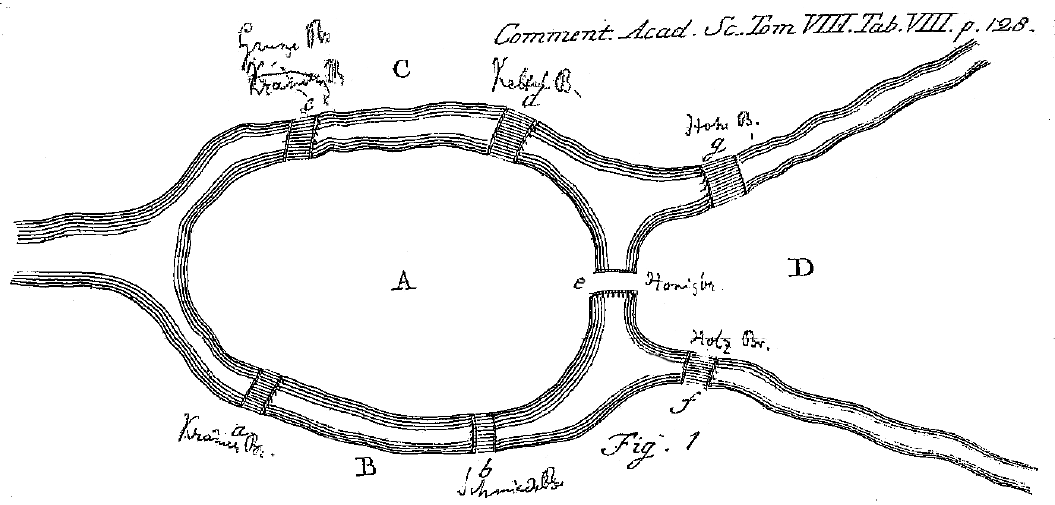
\includegraphics[width=\textwidth]{images/ex__konigsberg_bridges__schematic__drawing}
      \caption{The first figure from Euler's paper \cite{Euler1741}.}
      \label{fig:ex:konigsberg_bridges/schematic/drawing}
    \end{subcaptionblock}
    \hfill
    \begin{subcaptionblock}{0.4\textwidth}
      \centering
      \begin{equation}\label{eq:fig:ex:konigsberg_bridges/schematic/graph}
        \includegraphics{output/ex__konigsberg_bridges}
      \end{equation}
      \caption{The corresponding \hyperref[def:undirected_multigraph]{undirected multigraph}.}
      \label{fig:ex:konigsberg_bridges/schematic/graph}
    \end{subcaptionblock}

    \caption{Schematic drawings of the \hyperref[ex:konigsberg_bridges]{K\"onigsberg bridges puzzle}.}\label{fig:ex:konigsberg_bridges/schematic}
  \end{figure}

  Using sequences of letters, Euler manages to reformulate the puzzle in \S 7:
  \begin{displayquote}
    The problem is therefore reduced to finding a sequence of eight letters, formed from the four letters \( A \), \( B \), \( C \) and \( D \), in which the various pairs of letters occur the required number of times. Before I turn to the problem of finding such a sequence, it would be useful to find out whether or not it is even possible to arrange the letters in this way, for if it were possible to show that there is no such arrangement, then any work directed towards finding it would be wasted. I have therefore tried to find a rule which will be useful in this case, and in others, for determining whether or not such an arrangement can exist.
  \end{displayquote}

  Euler then deduces \fullref{thm:odd_degree_vertices} in \S 16 and \S 17 and further proceeds to deduce the following rule in \S 20:
  \begin{displayquote}
    If there are more than two areas to which an odd number of bridges lead, then such a journey is impossible.

    If, however, the number of bridges is odd for exactly two areas, then the journey is possible if it starts in either of these areas.

    If, finally, there are no areas to which an odd number of bridges leads, then the required journey can be accomplished starting from any area
  \end{displayquote}

  Therefore, the K\"onigsberg bridge puzzle is resolved negatively --- no route exists that can cross each bridge in \cref{fig:ex:konigsberg_bridges/schematic/drawing} exactly once. In modern terminology, the corresponding \hyperref[def:undirected_multigraph]{undirected multigraph} \eqref{eq:fig:ex:konigsberg_bridges/schematic/graph} has no \hyperref[def:walk/closed]{closed} \hyperref[def:eulerian_walk]{Eulerian walk} because it all of its vertices have odd \hyperref[def:graph_cardinality/undirected_degree]{degree}.

  Euler's general result is formulated with modern rigor and modern terminology and is proved in \fullref{thm:eulers_theorem_for_graphs}.
\end{example}

\paragraph{Four kinds of graphs}\hfill

The term \enquote{graph} is unfortunately very ambiguous\fnote{The graph of a relation or function is unrelated to the combinatorial graphs discussed here.} - it is a set of vertices connected by either directed arcs or undirected edges. \incite[362]{Knuth1997Vol1} states the following:
\begin{displayquote}
  Unfortunately, there will probably never be a standard terminology in this field, and so the author has followed the usual practice of contemporary books on graph theory, namely to use words that are similar but not identical to the terms used in any other books on graph theory.
\end{displayquote}

 We introduce distinct definitions for the four types of graphs from \cref{fig:def:graph_functors}, along with comments on how the definitions are used by different authors, and then in \fullref{def:graph_functors} we will define functors that help transparently transform some types of graphs into others. It is an established convention to not go through these hoops and implicitly transfer concepts between different kinds of graphs without even mentioning morphisms and categories. We will later follow this convention, but will nonetheless first describe the details.

\begin{figure}[!ht]
  \caption{Functors between the categories of different kinds of graphs.}\label{fig:def:graph_functors}
  \smallskip
  \hfill
  \begin{tikzpicture}
    \node[align=center] (dm) at (0, 0) {\hyperref[def:directed_graph/category]{Simple} \\ \hyperref[def:directed_graph/category]{directed} \\ \hyperref[def:directed_graph/category]{graphs} \\ {\scriptsize \hyperref[def:directed_graph/category]{(with loops)}}};
    \node[align=center] (um) at (5cm, 0) {\hyperref[def:undirected_graph/category]{Simple} \\ \hyperref[def:undirected_graph/category]{undirected} \\ \hyperref[def:undirected_graph/category]{graphs} \\ {\scriptsize \hyperref[def:undirected_graph/category]{(with loops)}}};
    \node[align=center] (ds) at (0, -3cm) {\hyperref[def:directed_multigraph/category]{Directed} \\ \hyperref[def:directed_multigraph/category]{multigraphs}};
    \node[align=center] (us) at (5cm, -3cm) {\hyperref[def:undirected_multigraph/category]{Undirected} \\ \hyperref[def:undirected_multigraph/category]{multigraphs}};
    \draw[->] (dm) to node[midway, above] {\hyperref[def:graph_functors/multi_forgetful]{\( U_S \)}} (um);
    \draw[->, bend left] (um) to node[midway, below] {\hyperref[def:graph_functors/simple_doubling]{\( D_S \)}} (dm);
    \draw[->] (ds) to node[midway, below] {\hyperref[def:graph_functors/multi_forgetful]{\( U_M \)}} (us);
    \draw[->, bend left] (dm) to node[midway, right] {\hyperref[def:graph_functors/directed_forgetful]{\( U_D \)}} (ds);
    \draw[->, bend left] (ds) to node[midway, left] {\hyperref[def:graph_functors/directed_inclusion]{\( I_D \)}} (dm);
    \draw[->, bend left] (um) to node[midway, right] {\hyperref[def:graph_functors/undirected_forgetful]{\( U_U \)}} (us);
    \draw[->, bend left] (us) to node[midway, left] {\hyperref[def:graph_functors/undirected_inclusion]{\( I_U \)}} (um);
  \end{tikzpicture}
  \hfill\hfill
\end{figure}

\begin{definition}\label{def:directed_multigraph}\mcite[def. 1.1.1; def. 1.1.2]{Knauer2011}
  A \term[bg=ориентиран (\cite[6]{Мирчев2001}) мултиграф (\cite[7]{Мирчев2001}), ru=ориентированый мультиграф (\cite[16]{Емеличев1990})]{directed multigraph} \( G \) consists of the following:
  \begin{thmenum}[series=def:directed_multigraph]
    \thmitem{def:directed_multigraph/vertices} A set \( V_G \), whose elements we call \term[bg=върхове (\cite[6]{Мирчев2001}), ru=вершины (\cite[279]{Емеличев1990})]{vertices}.

    \thmitem{def:directed_multigraph/arcs} A disjoint from \( V_G \) set \( A_G \), whose elements we call \term[bg=дъги (\cite[6]{Мирчев2001}), ru=дуги (\cite[279]{Емеличев1990})]{arcs}.
    \thmitem{def:directed_multigraph/head} A function \( h_G: A \to V \), giving the \term[en=head (\cite[544]{Rosen1999})]{head} or \term[bg=начален връх (\cite[7]{Мирчев2001}), ru=начало (\cite[279]{Емеличев1990}), en=initial vertex (\cite[28]{Diestel2005})]{initial endpoint} of an arc.

    \thmitem{def:directed_multigraph/tail} A function \( t_G: A \to V \), giving the \term[en=tail (\cite[544]{Rosen1999})]{tail} or \term[bg=краен връх (\cite[7]{Мирчев2001}), ru=конец (\cite[279]{Емеличев1990}), en=terminal vertex (\cite[28]{Diestel2005})]{terminal endpoint} of an arc.
  \end{thmenum}

  \Cref{fig:def:directed_multigraph} illustrates this definition. The figure is not merely schematic --- it is a \hyperref[def:graph_geometric_realization/embedding]{graph embedding}.

  \begin{figure}[!ht]
    \begin{equation}\label{eq:fig:def:directed_multigraph}
      \begin{aligned}
        \includegraphics[page=1]{output/def__directed_multigraph}
      \end{aligned}
    \end{equation}
    \caption{A \hyperref[def:directed_multigraph]{directed multigraph} with a pair of parallel arcs, a pair of oppositely directed arcs and a loop. Removing the dashed arcs makes it a \hyperref[def:directed_graph]{simple directed graph}.}\label{fig:def:directed_multigraph}
  \end{figure}

  We will need the following basic notions:
  \begin{thmenum}[resume=def:directed_multigraph]
    \thmitem{def:directed_multigraph/loop} We call the arc \( e \) a \term[bg=примка (\cite[7]{Мирчев2001}), ru=петля (\cite[279]{Емеличев1990})]{loop} if \( h(e) = t(e) \).

    \medskip

    \thmitem{def:directed_multigraph/parallel}\mcite[28]{Diestel2005} We call the arcs \( e \) and \( f \) \term[bg=паралелни (ребра) (\cite[7]{Мирчев2001}), ru=параллельные (рёбра) (\cite[279]{Емеличев1990})]{parallel} if \( h(e) = h(f) \) and \( t(e) = t(f) \) and \term{opposite} if it is not a loop and \( h(e) = t(f) \) and \( t(e) = h(f) \).

    \thmitem{def:directed_multigraph/homomorphism}\mcite[def. 1.4.1]{Knauer2011} A \term{homomorphism} between directed multigraphs \( G \) and \( H \) is a pair of functions
    \begin{align*}
      &f_V: V_G \to V_H, \\
      &f_A: A_G \to A_H,
    \end{align*}
    such that
    \begin{subequations}
      \begin{align}
        h_H \bincirc f_A &= f_V \bincirc h_G, \label{eq:def:directed_multigraph/homomorphism/head} \\
        t_H \bincirc f_A &= f_V \bincirc t_G. \label{eq:def:directed_multigraph/homomorphism/tail}
      \end{align}
    \end{subequations}

    Isomorphisms are discussed in \fullref{thm:graph_isomorphisms/multi_directed}.

    \thmitem{def:directed_multigraph/category}\mcite[48]{MacLane1998} Given a Grothendieck universe \( \mscrU \), we can define the \hyperref[def:category]{category} of \( \mscrU \)-small directed multigraphs as follows:
    \begin{itemize}
      \item The \hyperref[def:category/objects]{set of objects} is the family of directed multigraphs, where both the set of vertices and the set of arcs are \( \mscrU \)-small.

      \item The \hyperref[def:category/morphisms]{morphisms} between two directed multigraphs are their homomorphisms as defined in \fullref{def:directed_multigraph/homomorphism}.

      \item The \hyperref[def:category/composition]{composition of the morphisms} \( (f_V, f_A): G \to H \) and \( (g_V, g_A): H \to K \) is their componentwise function composition
      \begin{equation*}
        (g_V \bincirc f_V, g_A \bincirc f_A): G \to K.
      \end{equation*}

      \item The \hyperref[def:category/identity]{identity morphism} on the directed multigraph \( G \) is \( (\id_{V_G}, \id_{A_G}) \).
    \end{itemize}

    \thmitem{def:directed_multigraph/subgraph}\mcite[3]{Diestel2005} We say that \( H \) is a \term{subgraph} of \( G \) if \( V_G \subseteq V_H \), \( A_G \subseteq A_H \) and \( h_H \) and \( t_H \) are restrictions of \( h_G \) and \( t_G \) to \( A_H \).
  \end{thmenum}
\end{definition}
\begin{comments}
  \item Formally, we define a directed multigraph as a quadruple \( G = (V_G, A_G, h_G, t_G) \). We may skip indices when unnecessary, i.e. we are free to write \( G = (V, A, h, t) \) or even \( H = (W, B, j, u) \).

  \item \incite[def. 1.1.1]{Knauer2011}, \incite[10]{MacLane1998} and \incite[28]{Diestel2005} provide definitions similar to ours, but call them \enquote{directed graphs}. Knauer later distinguishes between simple and multigraphs, while Diestel uses \enquote{oriented graph} for what we call \enquote{simple directed graph}. \incite[8]{Bollobas1998} briefly mentions directed multigraphs and calls them as such.

  Diestel and Bollobas reserve the term \enquote{multigraph} for \hyperref[def:undirected_multigraph]{undirected multigraphs}. The latter also implicitly restricts graphs to finite order. These two books use \hyperref[def:undirected_graph]{simple undirected graphs} almost exclusively.
\end{comments}

\begin{remark}\label{rem:digraph}
  The term \enquote{digraph} is used as a shorthand for \enquote{directed graph}, for example by \incite[10]{Harary1969}, \incite[def. 1.1.1]{Knauer2011}, \incite[372]{Knuth1997Vol1} and \incite[559]{Rosen1999}. \incite[28]{Diestel2005} also uses this terminology, and in his usage \enquote{graph} exclusively refers to \enquote{undirected graph}.

  Similarly, in Russian, \enquote{орграф} is used as a shorthand for \enquote{ориентированный граф}, for example by \incite[\S 7.1.5]{Новиков2013} or \incite[279]{Емеличев1990}.

  We avoid the term.
\end{remark}

\begin{remark}\label{rem:subgraphs_and_subobjects}
  Subgraphs are not \hyperref[def:subobject_and_quotient]{categorical subobjects} because a graph can have distinct \hyperref[thm:graph_isomorphism]{isomorphic} subgraphs. For example, all one-vertex subgraphs are isomorphic, but nonetheless we consider them to be different subgraphs.
\end{remark}

\begin{definition}\label{def:directed_graph}\mcite[def. 1.1.2]{Knauer2011}
  A \term{simple directed graph} \( G \) consists of the following:
  \begin{thmenum}[series=def:directed_graph]
    \thmitem{def:directed_graph/vertices} A set \( V_G \), whose elements we call \term{vertices}.
    \thmitem{def:directed_graph/arcs} A disjoint from \( V_G \) set \( A_G \) of \hyperref[def:cartesian_product/kuratowski_pair]{ordered pairs} of \hi{distinct} vertices. As in the case of directed multigraphs, we call the elements of \( A_G \) \term{arcs}. If we allow vertices whose endpoints coincide, we will say that \( G \) is a \enquote{simple directed graph, possibly with loops}.
  \end{thmenum}

  Simple directed graphs have the following metamathematical properties:
  \begin{thmenum}[resume=def:directed_graph]
    \thmitem{def:directed_graph/theory}\mimprovised We can regard directed graphs as models of a \hyperref[def:first_order_theory]{first-order theory} over a \hyperref[def:first_order_signature]{first-order signature} \( \Sigma \) with a single \hyperref[rem:first_order_formula_conventions/infix]{infix} predicate symbol, possibly with the irreflexivity axiom \eqref{eq:def:binary_relation/irreflexive}.

    \thmitem{def:directed_graph/homomorphism}\mimprovised A \hyperref[def:first_order_homomorphism]{first-order homomorphism} between the \( G \) and \( H \) is a function \( f: V_G \to V_H \) such that \( (u, v) \in A_G \) implies \( (f(u), f(v)) \in A_H \).

    Isomorphisms are discussed in \fullref{thm:graph_isomorphisms/simple_directed}.

    \thmitem{def:directed_graph/category}\mimprovised Given a Grothendieck universe \( \mscrU \), we can define the \hyperref[def:category]{category} of \( \mscrU \)-small simple directed graphs, possibly with loops, and their homomorphisms. Disallowing loops leads to a full subcategory.

    \thmitem{def:directed_graph/subgraph}\mimprovised We say that \( H \) is a \term{subgraph} of \( G \) if \( V_G \subseteq V_H \) and \( A_G \subseteq A_H \).
  \end{thmenum}
\end{definition}
\begin{comments}
  \item We can regard directed graphs as directed multigraphs without loops and parallel arcs. This is made precise via the inclusion functor \hyperref[def:graph_functors/directed_inclusion]{\( I_D \)}.
\end{comments}

\begin{definition}\label{def:undirected_multigraph}\mcite[def. 1.1.2]{Knauer2011}
  An \term{undirected multigraph} \( G \) consists of the following:
  \begin{thmenum}[series=def:undirected_multigraph]
    \thmitem{def:undirected_multigraph/vertices} A set \( V_G \), whose elements we call \term{vertices}.
    \thmitem{def:undirected_multigraph/edges} A disjoint from \( V_G \) set \( E_G \), whose elements we call \term[bg=ребра (\cite[6]{Мирчев2001}), ru=рёбра (\cite[277]{БелоусовТкачёв2004})]{edges}.
    \thmitem{def:undirected_multigraph/endpoints} A map
    \begin{equation*}
      \mscrE: E \to \set[\Big]{ \set{ u, v } \given* u, v \in V },
    \end{equation*}
    giving an unordered pair of \term{endpoints} of an edge.
  \end{thmenum}

  \begin{figure}[!ht]
    \begin{equation}\label{eq:fig:def:undirected_multigraph}
      \begin{aligned}
        \includegraphics[page=1]{output/def__undirected_multigraph}
      \end{aligned}
    \end{equation}
    \caption{An undirected multigraph, which becomes simple after removing the dashed edges.}\label{fig:def:undirected_multigraph}
  \end{figure}

  We will use the following basic terminology:
  \begin{thmenum}[resume=def:undirected_multigraph]
    \thmitem{def:undirected_multigraph/loop} We call the edge \( e \) a \term{loop} if \( \mscrE(e) \) is a one-element set.

    \medskip

    \thmitem{def:undirected_multigraph/parallel} We call the edges \( e \) and \( f \) \term{parallel} if \( \mscrE(e) = \mscrE(f) \).

    \thmitem{def:undirected_multigraph/homomorphism}\mimprovised A \term{homomorphism} between the undirected multigraphs \( G \) and \( H \) is a pair of functions
    \begin{align*}
      &f_V: V_G \to V_H, \\
      &f_E: E_G \to E_H,
    \end{align*}
    such that, for each edge \( e \in E_G \),
    \begin{equation}\label{eq:def:undirected_multigraph/homomorphism}
      \mscrE_H(f_E(e)) = \set[\Big]{ f_V(v) \given* v \in \mscrE_G(e) }.
    \end{equation}

    Isomorphisms are discussed in \fullref{thm:graph_isomorphisms/multi_undirected}.

    \thmitem{def:undirected_multigraph/category}\mimprovised Given a Grothendieck universe \( \mscrU \), we can define the \hyperref[def:category]{category} of \( \mscrU \)-small undirected multigraphs and their homomorphisms.

    \thmitem{def:undirected_multigraph/subgraph}\mimprovised We say that \( H \) is a \term{subgraph} of \( G \) if \( V_G \subseteq V_H \), \( E_G \subseteq E_H \) and \( \mscrE_H = \mscrE_G\restr_{E_H} \).
  \end{thmenum}
\end{definition}
\begin{comments}
  \item \incite[def. 1.1.2]{Knauer2011} does not explicitly mention undirected multigraphs, but their existence is implied.

  \incite[10]{Harary1969}, \incite[28]{Diestel2005} and \incite[6]{Bollobas1998} define undirected multigraphs, although all omit the prefix \enquote{undirected}. Harary disallows loops, instead referring to multigraphs with loops as \enquote{pseudographs}. Bollobas explicitly defines directed multigraphs, while \incite[28]{Diestel2005} uses the term \enquote{directed graph} for what we call a \hyperref[def:directed_multigraph]{directed multigraph} and \enquote{oriented graph} for what we call \enquote{simple directed graph}.

  \incite[3]{GondranMinoux1984Graphs} define multigraphs without specifying whether they are directed or not, but later implicitly assume that they are undirected.
\end{comments}

\begin{definition}\label{def:undirected_graph}\mcite[3]{Diestel2005}
  A \term{simple undirected graph} \( G \) consists of the following:
  \begin{thmenum}[series=def:undirected_graph]
    \thmitem{def:undirected_graph/vertices} A set \( V_G \), whose elements we call \term{vertices}.
    \thmitem{def:undirected_graph/edges} A disjoint from \( V_G \) set \( E_G \) of unordered pairs of \hi{distinct} vertices, i.e. sets of the form \( \set{ u, v } \), whose elements we call \term{edges}. If we allow vertices whose endpoints coincide, we will say that \( G \) is a \enquote{simple undirected graph, possibly with loops}.
  \end{thmenum}

  We will use the following basic terminology:
  \begin{thmenum}[resume=def:undirected_graph]
    \thmitem{def:undirected_graph/homomorphism}\mcite[def. 1.4.3]{Knauer2011} A \term{homomorphism} between the simple undirected graphs \( G \) and \( H \) is a function \( f: V_G \to V_H \) such that \( \set{ u, v } \in E_G \) implies \( \set{ f(u), f(v) } \in E_H \).

    Isomorphisms are discussed in \fullref{thm:graph_isomorphisms/simple_undirected}.

    \thmitem{def:undirected_graph/category}\mcite[example 3.1.12]{Knauer2011} Given a Grothendieck universe \( \mscrU \), we can define the \hyperref[def:category]{category} of \( \mscrU \)-small simple undirected graphs, possibly with loops, and their homomorphisms. Disallowing loops leads to a full subcategory.

    By \fullref{thm:edgeless_graph_universal_property}, the monomorphisms are precisely the injective homomorphisms and, by \fullref{thm:complete_graph_universal_property}, the epimorphisms are precisely the surjective homomorphisms.

    \thmitem{def:undirected_graph/subgraph}\mcite[3]{Diestel2005} We say that \( H \) is a \term{subgraph} of \( G \) if \( V_G \subseteq V_H \) and \( E_G \subseteq E_H \).
  \end{thmenum}
\end{definition}
\begin{comments}
  \item We can regard undirected graphs as undirected multigraphs without loops and parallel arcs. This is made precise via the inclusion functor \hyperref[def:graph_functors/undirected_inclusion]{\( I_U \)}.

  \item \incite[9]{Harary1969}, \incite[2]{Diestel2005} and \incite[1]{Bollobas1998} define simple undirected graphs similarly to how we have done it. \incite[def. 1.1.2]{Knauer2011} also does, however he allows loops.

  \item \incite[def. 1.4.8]{Knauer2011} define subgraphs more generally as graphs which can be embedded via injective graph homomorphisms. We prefer the vertices and edges of subgraphs to be subsets.
\end{comments}

\begin{remark}\label{rem:theory_of_simple_undirected_graphs}
  For the purpose of fitting \hyperref[def:undirected_graph]{simple undirected graphs} in the framework of first-order logic, we can extend the \hyperref[def:directed_graph/theory]{theory of directed graphs} with the symmetry axiom \eqref{eq:def:binary_relation/symmetry}.

  This leads to an incompatible notion of homomorphisms, however --- the \hyperref[def:first_order_homomorphism]{first-order homomorphisms} of this theory are the directed graph homomorphisms defined in \fullref{def:directed_graph/homomorphism} and not the more general undirected graph homomorphisms defined in \fullref{def:undirected_graph/homomorphism}.

  We will still find this theory useful, for example when defining quotient graphs in \fullref{def:quotient_graph}.
\end{remark}

\begin{remark}\label{rem:simple_graphs}
  Whether or simple graphs are allowed have loops again depends on the authors.

  Defining \enquote{directed graphs} as pairs \( (V, A) \), where \( A \subseteq V \times V \), without further restrictions, is common. It is done by \incite[10]{Harary1969}, \incite[def. 1.1.2]{Knauer2011}, \incite[21]{GondranMinoux1984Graphs}, \incite[10]{Savage1998}, \incite[190]{Erickson2019}, \incite[279]{Емеличев1990}, \incite[277]{БелоусовТкачёв2004} and \incite[6]{Мирчев2001}. \incite[\S 7.1.5]{Новиков2013} also provides the same definition, however he forbids loops unless explicitly mentioned. \incite[39]{Diestel2005} uses the term \enquote{oriented graph} for what we call \enquote{simple directed graph}.

  For undirected graphs we instead have several conventions:
  \begin{itemize}
    \item Some of the aforementioned authors, namely \incite[21]{GondranMinoux1984Graphs}, \incite[10]{Savage1998} and \incite[277]{БелоусовТкачёв2004}, define directed graphs as \enquote{symmetric} undirected graphs, in which \( (u, v) \) is an arc whenever \( (v, u) \) is. This definition allows loops since the directed counterparts do.

    \item Other aforementioned authors, namely \incite[def. 1.1.2]{Knauer2011}, \incite[190]{Erickson2019}, and \incite[7]{Мирчев2001} define undirected graphs as pairs \( (V, E) \), where \( E \) consists of one-element or two-element subsets of \( V \). This definition again allows loops.

    \item \incite[9]{Harary1969}, \incite[2]{Diestel2005}, \incite[1]{Bollobas1998}, \incite[9]{Емеличев1990} and \incite[\S 7.1.2]{Новиков2013} define directed graphs as pairs \( (V, E) \), where \( E \) consists of two-element subsets of \( V \). This explicitly forbid loops.

    \item \incite[377]{Knuth1997Vol1} explicitly forbids loops in graphs, however he defines \enquote{graphs} as \enquote{a set of points together with a set of lines}.
  \end{itemize}

  \incite[def. 1.1.2]{Knauer2011} uses the adjective \enquote{simple} to refer to (multi)graphs without multiple edges, without referring to loops. So do \incite[2]{Diestel2005} and \incite[22]{Bollobas1998}, however their definitions of graphs forbid loops by default. \incite[22]{GondranMinoux1984Graphs}, \incite[191]{Erickson2019}, \incite[540]{Rosen1999}, \incite[17]{Емеличев1990} and \incite[12]{Мирчев2001} use \enquote{simple} to additionally forbid loops.

  We prefer our terminology to be as unambiguous as possible, for which reason we use \enquote{simple} in the latter sense and, if loops are allowed, we mention it explicitly.
\end{remark}

\begin{proposition}\label{thm:graph_isomorphisms}
  In order to discuss graph isomorphisms systematically, we study \hyperref[def:morphism_invertibility/isomorphism]{categorical isomorphisms} on their respective categories.

  \begin{thmenum}
    \thmitem{thm:graph_isomorphisms/multi_directed} Given \hyperref[def:directed_multigraph]{directed multigraphs} \( G \) and \( H \), the \hyperref[def:directed_multigraph/homomorphism]{directed multigraph homomorphism}
    \begin{align*}
      &f_V: V_G \to V_H, \\
      &f_A: A_G \to A_H,
    \end{align*}
    is a categorical isomorphism if and only if both \( f_V \) and \( f_A \) are bijective.

    Furthermore, the componentwise inverse \( (f_V^{-1}, f_A^{-1}) \) of \( (f_V, f_A) \) is also a homomorphism, and it is the two-sided inverse of \( (f_V, f_A) \) in the category of directed multigraphs.

    \thmitem{thm:graph_isomorphisms/simple_directed} Given \hyperref[def:directed_graph]{simple directed graphs} \( G \) and \( H \), possibly with loops, the \hyperref[def:directed_graph/homomorphism]{directed graph homomorphism} \( f: V_G \to V_H \) is a categorical isomorphism if and only if it is bijective and satisfies
    \begin{equation}\label{eq:thm:graph_isomorphisms/simple_directed}
      (u, v) \in A_G \T{if and only if} (f(u), f(v)) \in A_H.
    \end{equation}

    Furthermore, the inverse function \( f^{-1} \) of \( f \) is also a homomorphism, it satisfies \eqref{eq:thm:graph_isomorphisms/simple_directed}, and it is the two-sided inverse of \( f \) in the category of simple directed graphs.

    \thmitem{thm:graph_isomorphisms/multi_undirected} Given \hyperref[def:undirected_multigraph]{undirected multigraphs} \( G \) and \( H \), the \hyperref[def:undirected_multigraph/homomorphism]{undirected multigraph homomorphism}
    \begin{align*}
      &f_V: V_G \to V_H, \\
      &f_E: E_G \to E_H,
    \end{align*}
    is a categorical isomorphism if and only if both \( f_V \) and \( f_E \) are bijective.

    Furthermore, the componentwise inverse \( (f_V^{-1}, f_E^{-1}) \) of \( (f_V, f_E) \) is also a homomorphism, and it is the two-sided inverse of \( (f_V, f_E) \) in the category of directed multigraphs.

    \thmitem{thm:graph_isomorphisms/simple_undirected} Given \hyperref[def:undirected_graph]{simple undirected graphs} \( G \) and \( H \), possibly with loops, the \hyperref[def:undirected_graph/homomorphism]{undirected graph homomorphism} \( f: V_G \to V_H \) is a categorical isomorphism if and only if it is bijective and satisfies
    \begin{equation}\label{eq:thm:graph_isomorphisms/simple_undirected}
      \set{ u, v } \in E_G \T{if and only if} \set{ f(u), f(v) } \in E_H.
    \end{equation}
  \end{thmenum}
\end{proposition}
\begin{comments}
  \item \incite[583]{Rosen1999} uses our characterizations as definitions. \incite[3]{Diestel2005}, \incite[3]{Bollobas1998}, \incite[def. 4.1.3]{Knauer2011}, \incite[13]{Емеличев1990} and \incite[def. 5.14]{БелоусовТкачёв2004}, \incite[\S 7.1.6]{Новиков2013} define simple undirected graph isomorphisms via \eqref{eq:thm:graph_isomorphisms/simple_undirected}, however avoid discussing isomorphisms for other kinds of graphs.
\end{comments}
\begin{proof}
  \SubProofOf{thm:graph_isomorphisms/multi_directed}

  \SufficiencySubProof* Suppose that \( (f_V, f_A): G \to H \) is a categorical isomorphism. Clearly it is a homomorphism. We must show that both \( f_V \) and \( f_A \) are bijective.

  We have two forgetful functors into \( \cat{Set} \) --- one for vertices and functions between them, the other one for arcs and functions between them. Hence, by \fullref{thm:def:functor_invertibility/preserves_inverses}, both \( f_V \) and \( f_A \) are set isomorphisms, and, by \fullref{thm:function_invertibility_categorical/fully_invertible}, both are bijective.

  \NecessitySubProof* Suppose that \( (f_V, f_A): G \to H \) is a homomorphism and that both \( f_V \) and \( f_A \) are bijective. We will show that \( (f_V^{-1}, f_A^{-1}) \) is a homomorphism from \( H \) to \( G \).

  For any arc \( e \) in \( H \), we have
  \begin{equation*}
    f_V(h_G(f^{-1}_A(e)))
    \reloset {\eqref{eq:def:directed_multigraph/homomorphism/head}} =
    h_H(f_A(f^{-1}_A(e)))
    =
    h_H(e),
  \end{equation*}
  hence
  \begin{equation*}
    h_G(f^{-1}_A(e))
    =
    f_V^{-1}(f_V(h_G(f^{-1}_A(e))))
    =
    f_V^{-1}(h_H(e)).
  \end{equation*}

  We can analogously show that
  \begin{equation*}
    t_G(f^{-1}_A(e)) = f_V^{-1}(t_H(e)).
  \end{equation*}

  Thus, the pair \( (f_V^{-1},f_A^{-1}) \) satisfies both \eqref{eq:def:directed_multigraph/homomorphism/head} and \eqref{eq:def:directed_multigraph/homomorphism/tail}, which makes it a directed multigraph homomorphism.

  Composing \( (f_V, f_A) \) and \( (f_V^{-1}, f_A^{-1}) \) (componentwise), we obtain identity homomorphisms on either \( G \) or \( H \) depending on the order of composition. Therefore, \( (f_V, f_A) \) is fully invertible, that is, a categorical isomorphism.

  \SubProofOf{thm:graph_isomorphisms/simple_directed}

  \SufficiencySubProof* Suppose that \( f: V_G \to V_H \) is a categorical isomorphism between \( G \) and \( H \). Again, by \fullref{thm:def:functor_invertibility/preserves_inverses}, \( f \) is an isomorphism between \( V_G \) and \( V_H \) in the category of sets, that is, a bijective function.

  Let \( g: V_G \to V_H \) be the categorical inverse of \( f \). Then it is the inverse of \( f \) in \( \cat{Set} \), which due to the uniqueness of two-sided inverses implies that \( g \) is the inverse function \( f^{-1} \) of \( f \).

  Then, if \( (f(u), f(v)) \) is an arc of \( H \) for some vertices \( u \) and \( v \),
  \begin{equation*}
    \parens[\Big]{ f^{-1}(f(u)), f^{-1}(f(v)) } = (u, v)
  \end{equation*}
  is an edge of \( G \). Therefore, \eqref{eq:thm:graph_isomorphisms/simple_directed} holds.

  \NecessitySubProof* Suppose that \( f: V_G \to V_H \) is a bijective homomorphism from \( G \) to \( H \) and that \eqref{eq:thm:graph_isomorphisms/simple_directed} holds.

  For any arc \( (u, v) \) in \( H \), we have
  \begin{equation*}
    (u, v) = \parens[\Big]{ f(f^{-1}(u)), f(f^{-1}(v)) }.
  \end{equation*}
  and thus, by \eqref{eq:thm:graph_isomorphisms/simple_directed}, \( (f^{-1}(u), f^{-1}(v)) \) is an arc in \( G \).

  Therefore, \( f^{-1} \) is itself a homomorphism from \( H \) to \( G \), and it clearly satisfies \eqref{eq:thm:graph_isomorphisms/simple_directed}. When composed with \( f \), we obtain the identity on either \( V_G \) or \( V_H \) depending on the order of composition, hence \( f^{-1} \) is the two-sided inverse of \( f \).

  \SubProofOf{thm:graph_isomorphisms/multi_undirected}

  \SufficiencySubProof* If \( (f_V, f_E): G \to H \) is a categorical isomorphism, we can prove that both \( f_V \) and \( f_E \) are bijective analogously to the case for directed multigraphs.

  \NecessitySubProof* Suppose that \( (f_V, f_E): G \to H \) is a homomorphism and that both \( f_V \) and \( f_E \) are bijective.

  For any edge \( e \) of \( H \), we have
  \begin{equation*}
    \mscrE_H(e)
    =
    \mscrE_H\parens[\Big]{ f_E(f_E^{-1}(e)) }
    \reloset {\eqref{eq:def:undirected_multigraph/homomorphism}} =
    \set{ f_V(u) \given u in \mscrE_G(f_E^{-1}(e)) }.
  \end{equation*}

  Then
  \begin{equation*}
    \set{ f_V^{-1}(v) \given v \in \mscrE_H(e) }
    =
    \set{ f_V^{-1}(f_V(u)) \given u \in \mscrE_G(f_E^{-1}(e)) }
    =
    \mscrE_G(f_E^{-1}(e)).
  \end{equation*}

  Therefore, the pair \( (f_V^{-1}, f_E^{-1}) \) satisfies \eqref{eq:def:undirected_multigraph/homomorphism}, which makes it a homomorphism of undirected multigraphs.

  Analogously to the case of directed multigraphs, we conclude that \( (f_V, f_E) \) is a categorical isomorphism with inverse \( (f_V^{-1}, f_E^{-1}) \).

  \SubProofOf{thm:graph_isomorphisms/simple_undirected} Both sufficiency and necessity can be proven similarly to the case of simple directed graphs.
\end{proof}

\begin{definition}\label{def:multigraph_orientation}\mcite[def. 6.2.1]{Knauer2011}
  We call the \hyperref[def:directed_multigraph]{directed multigraph} \( D = (V, A, h, t) \) an \term[ru=ориентация (\cite[32]{Емеличев1990})]{orientation} of the \hyperref[def:undirected_multigraph]{undirected multigraph} \( G = (U, E, \mscrE) \) if \( U = V \), \( A = E \), and, for every arc \( e \in A \), we have \( \mscrE(e) = \set{ h(e), t(e) } \).
\end{definition}
\begin{comments}
  \item This definition also applies to simple graphs via the inclusion functors \hyperref[def:graph_functors/directed_inclusion]{\( I_D \)} and \hyperref[def:graph_functors/undirected_inclusion]{\( I_U \)}.
\end{comments}

\begin{definition}\label{def:graph_functors}\mimprovised
  Different kinds of graphs are related via the following functors (shown graphically in \fullref{fig:def:graph_functors}):
  \begin{thmenum}
    \thmitem{def:graph_functors/directed_forgetful} The simple \hyperref[def:concrete_category]{forgetful functor}:
    \begin{flalign*}
      &U_D: \hyperref[def:directed_multigraph/category]{\T*{Directed multigraphs}} \to \hyperref[def:directed_graph/category]{\T*{Simple directed graphs with loops}}, &&\\
      &U_D(V, A, h, t) \coloneqq \parens[\Big]{ V, \set[\Big]{ \parens[\Big]{ h(a), t(a) } \given* a \in A } }, &&\\
      &U_D(f_V, f_A) \coloneqq f_V.
    \end{flalign*}

    \thmitem{def:graph_functors/directed_inclusion} A \hyperref[def:category_adjunction]{left adjoint}:
    \begin{flalign*}
      &I_D: \hyperref[def:directed_graph/category]{\T*{Simple directed graphs}} \to \hyperref[def:directed_multigraph/category]{\T*{Directed multigraphs}}, &&\\
      &I_D(V, A) \coloneqq \parens[\Big]{ V, A, (u, v) \mapsto u, (u, v) \mapsto v }, &&\\
      &I_D(f) \coloneqq \parens[\Big]{ f, (u, v) \mapsto \parens[\Big]{ f(u), f(v) } }.
    \end{flalign*}

    \thmitem{def:graph_functors/undirected_forgetful} A similar forgetful functor for undirected graphs:
    \begin{flalign*}
      &U_U: \hyperref[def:undirected_multigraph/category]{\T*{Undirected multigraphs}} \to \hyperref[def:undirected_graph/category]{\T*{Simple undirected graphs with loops}}, &&\\
      &U_U(V, E, \mscrE) \coloneqq \parens[\Big]{ V, \set[\Big]{ \mscrE(e) \given* e \in E } }, &&\\
      &U_U(f_V, f_E) \coloneqq f_V.
    \end{flalign*}

    \thmitem{def:graph_functors/undirected_inclusion} A left adjoint:
    \begin{flalign*}
      &I_U: \hyperref[def:undirected_graph/category]{\T*{Simple undirected graphs}} \to \hyperref[def:undirected_multigraph/category]{\T*{Undirected multigraphs}}, &&\\
      &I_U(V, E) \coloneqq \parens[\Big]{ V, E, e \mapsto e }, &&\\
      &I_U(f) \coloneqq \parens[\Big]{ f, \set{ u, v } \mapsto \set{ f(u), f(v) } }.
    \end{flalign*}

    \thmitem{def:graph_functors/multi_forgetful} A functor that forgets the \hyperref[def:multigraph_orientation]{orientation} of a multigraph:
    \begin{flalign*}
      &U_M: \hyperref[def:directed_multigraph/category]{\T*{Directed multigraphs}} \to \hyperref[def:undirected_multigraph/category]{\T*{Undirected multigraphs}}, &&\\
      &U_M(V, A, h, t) \coloneqq \parens[\Big]{ V, A, e \mapsto \set{ h(e), t(e) } }, &&\\
      &U_M(f_V, f_A) \coloneqq (f_V, f_A).
    \end{flalign*}

    \thmitem{def:graph_functors/simple_forgetful} A functor that forgets the orientation of a simple graph:
    \begin{flalign*}
      &U_S: \hyperref[def:directed_graph/category]{\T*{Simple directed graphs}} \to \hyperref[def:undirected_graph/category]{\T*{Simple undirected multigraphs}}, &&\\
      &U_S(V, A) \coloneqq \parens[\Big]{ V, A, (u, v) \mapsto \set{ u, v } }, &&\\
      &U_S(f) \coloneqq f.
    \end{flalign*}

    Note that opposite arcs map to the same edge.

    \thmitem{def:graph_functors/simple_doubling} A right adjoint to \( U_S \), which doubles each edge to produce arcs in both directions:
    \begin{flalign*}
      &D_S: \hyperref[def:undirected_graph/category]{\T*{Simple undirected graphs}} \to \hyperref[def:directed_multigraph/category]{\T*{Simple directed graphs}}, &&\\
      &D_S(V, E) \coloneqq \parens[\Big]{ V, \set[\Big]{ (u, v) \in V^2 \given \set{ u, v } \in E } }, &&\\
      &D_S(f) \coloneqq f.
    \end{flalign*}
  \end{thmenum}
\end{definition}
\begin{comments}
  \item \Fullref{ex:def:category_adjunction/us_ds} discusses the doubling functor from \fullref{def:graph_functors/simple_doubling}.
  \item We can introduce a doubling functor for multigraphs similar to \hyperref[def:graph_functors/simple_doubling]{\( D_S \)} that introduces two opposite copies of each edge in an undirected multigraph.

  Unfortunately, that would require choosing one vertex as the head and the other as a tail, and thus the functor depends on a \hyperref[def:choice_function]{choice function}. This choice function is unnecessary for simple graphs because ordered pairs having a first and second element, while multigraphs have abstract objects as arcs.

  Furthermore, even given a canonical choice function, this functor would not be a right inverse to \hyperref[def:graph_functors/multi_forgetful]{\( U_M \)} --- instead, we would obtain an undirected multigraph with twice as many edges as the original.

  We avoid introducing such a functor altogether.
\end{comments}

\begin{remark}\label{rem:arbitrary_kind_graph}
  We will henceforth use the phrase \enquote{arbitrary-kind graph} to refer to any of the four kinds of graphs defined in this section.

  The inclusion functors \hyperref[def:graph_functors/directed_inclusion]{\( I_D \)} and \hyperref[def:graph_functors/undirected_inclusion]{\( I_U \)} allow all definitions for multigraphs to apply to simple graphs. The transition between directed and undirected graphs is more complicated, but we will nonetheless utilize \hyperref[def:graph_functors/multi_forgetful]{\( U_M \)}, \hyperref[def:graph_functors/simple_forgetful]{\( U_S \)} and \hyperref[def:graph_functors/simple_doubling]{\( D_S \)} when necessary.

  These functors will be used implicitly, but when increased attention is required, we use these functors explicitly. See \fullref{thm:graph_coloring_as_homomorphism} for an example.
\end{remark}

\begin{definition}\label{def:induced_subgraph}\mcite[def. 1.4.8]{Knauer2011}
  In an \hyperref[rem:arbitrary_kind_graph]{arbitrary-kind graph} \( G \), for every set \( U \) of vertices, we define the \term[ru=порождённый (подграф) (\cite[17]{Емеличев1990}), bg=породен (подграф) (\cite[18]{Мирчев2001})]{induced subgraph} \( G[U] \) as the unique subgraph with vertex set \( U \) that contains all arcs/edges of \( G \) with endpoints in \( U \).
\end{definition}

\begin{definition}\label{def:graph_incidence}\mcite[def. 1.1.1]{Knauer2011}
  In an \hyperref[rem:arbitrary_kind_graph]{arbitrary-kind graph}, we say that the vertex \( v \) and the arc/edge \( e \) are \term[bg=инцидентни (ребра) (\cite[7]{Мирчев2001}), ru=инцидентные (рёбра) (\cite[9]{Емеличев1990})]{incident} of \( v \) is an endpoint of \( e \).
\end{definition}

\begin{definition}\label{def:graph_adjacency}\mcite[def. 1.1.8]{Knauer2011}
  In an \hyperref[rem:arbitrary_kind_graph]{arbitrary-kind graph}, if two vertices (resp. arcs/edges) are \hyperref[def:graph_incidence]{incident} to a common arc/edge (resp. vertex), we say that they are \term[bg=съседни (върхове/дъги/ребра) (\cite[7]{Мирчев2001}), ru=смежные (вершины/рёбра) (\cite[9]{Емеличев1990})]{adjacent}.
\end{definition}

\begin{definition}\label{def:graph_independent_set}\mcite[def. 1.4.12]{Knauer2011}
  We say that a subset of the vertices (resp. arcs/edges) of an \hyperref[rem:arbitrary_kind_graph]{arbitrary-kind graph} is an \term[bg=независимо множество (\cite[103]{Мирчев2001})]{independent set} if no two vertices (resp. arcs/edges) in it are \hyperref[def:graph_adjacency]{adjacent}.
\end{definition}

\begin{remark}\label{rem:trivial_graph}
  Unlike the \hyperref[def:group/trivial]{trivial group} \( \set{ e } \) or \hyperref[def:module/trivial]{trivial \( R \)-module} \( \set{ 0 } \), which are unique up to an isomorphism, there is no trivial graph in the sense of \fullref{def:trivial_object}.

  Every graph has a subgraph with \hyperref[def:graph_cardinality/order]{order} zero, and hence up to an isomorphism we have an order-zero graph (for every kind of graph discussed here).

  Another unambiguous concept is that of an edgeless graph. Every \hyperref[def:complete_graph]{complete graph} has \( 2^n \) edgeless subgraphs (one for each set of edges).
\end{remark}

\paragraph{Cardinalities in graphs}

\begin{definition}\label{def:graph_cardinality}
  Graphs have the following notions of \hyperref[thm:cardinality_existence]{cardinality}:
  \begin{thmenum}
    \thmitem{def:graph_cardinality/order}\mcite[2]{Diestel2005} We define the \term[ru=порядок (\cite[9]{Емеличев1990})]{order} \( \ord(G) \) of an \hyperref[rem:arbitrary_kind_graph]{arbitrary-kind graph} \( G \) as the (cardinal) number of vertices.

    For a simple graph, finitely many vertices imply finitely many arcs/edges, which justifies terminology like \enquote{finite simple graph}. For multigraphs, however, we will prefer being more concrete and use \enquote{finite-order (multi)graph}.

    \thmitem{def:graph_cardinality/directed_degree}\mcite[def. 1.1.7]{Knauer2011} We define the \term[bg=полустепен на изхода (\incite[8]{Мирчев2001}), ru=полустепень исхода (\cite[283]{Емеличев1990})]{out-degree} \( \deg_{\op{out}}(v) \) (resp. \term[bg=полустепен на входа (\incite[8]{Мирчев2001}), ru=полустепень захода (\cite[283]{Емеличев1990})]{in-degree} \( \deg_{\op{in}}(v) \)) of a vertex \( v \) in a \hyperref[def:directed_multigraph]{directed (multi)graph} as the (cardinal) number of arcs starting (resp. ending) at \( v \).

    We define the \term[bg=степен (\cite[8]{Мирчев2001}), ru=степень (\cite[283]{Емеличев1990})]{degree} \( \deg(v) \) of \( v \) as the sum of the two.

    \thmitem{def:graph_cardinality/undirected_degree}\mimprovised If the graph is undirected, consider the \hyperref[def:multiset]{multiset} of all edges incident to \( v \), with loops having multiplicity \( 2 \) and all other edges having multiplicity \( 1 \).

    We define the \term{degree} \( \deg(v) \) as the \hyperref[def:multiset/cardinality]{cardinality} of this multiset.

    \thmitem{def:graph_cardinality/local}\mcite[196]{Diestel2005} We say that a graph is \term{locally finite} (resp. \term{locally countable}) if the degree of any vertex is finite (resp. countable).
  \end{thmenum}
\end{definition}

\begin{proposition}\label{thm:degree_of_undirected_counterpart}
  The degree, in the sense of \fullref{def:graph_cardinality/directed_degree}, of a vertex \( v \) in a \hyperref[def:directed_multigraph]{directed multigraph} \( G \), is equal to the degree, in the sense of \fullref{def:graph_cardinality/undirected_degree}, of \( v \) in the undirected counterpart \( \hyperref[def:graph_functors/multi_forgetful]{U_M}(G) \) of \( G \).
\end{proposition}
\begin{comments}
  \item When proving statements about vertex degrees, it thus makes sense to prove it for undirected multigraphs, since it will then also automatically apply to directed graphs.
\end{comments}
\begin{proof}
  We have adjusted our definitions so that this holds.
\end{proof}

\begin{remark}\label{rem:counting_loops_twice}
  Loops may contribute either \( 1 \) or \( 2 \) towards the degree of a graph. This choice simplifies \fullref{thm:sum_of_endpoint_degrees} and hence \fullref{thm:sum_of_graph_degrees}, as well as \fullref{def:graph_cycle}, among others.

  We describe here several conventions.
  \begin{itemize}
    \item \incite[27]{Емеличев1990}, who diligently distinguish between directed and undirected graphs, defines degrees in (simple) directed graphs as sums of out-degrees and in-degrees, like we do, and in undirected graphs they, like us, count loops twice.

    \item \incite[277]{БелоусовТкачёв2004}, who also give separate definitions for directed and undirected graphs, also define degrees in (simple) directed graphs as sums of out-degrees and in-degrees, but for undirected graphs they avoid counting loops twice.

    \item \incite[544]{Rosen1999} defines the degree of a vertex similarly to us, however without referring to multisets.

    \item \incite[191]{Erickson2019} and \incite[8]{Мирчев2001} define degrees without counting loops twice for both directed and undirected graphs.

    \item \incite[def. 1.1.7]{Knauer2011} avoids defining \enquote{total} degrees for directed graphs, leaving only out-degrees and in-degrees. For undirected graphs, however, in \cite[def. 1.1.8]{Knauer2011} he defines the degree of a vertex \( v \) as the number of edges incident to \( v \), which without our multiset trick only counts loops once.

    \item \incite[372]{Knuth1997Vol1} also defines out-degrees and in-degrees, but avoids defining degrees for both directed and undirected graphs.

    \item \incite[8]{Bollobas1998} hints that loops should be counted twice.
  \end{itemize}
\end{remark}

\begin{definition}\label{def:isolated_vertex}\mcite[5]{Diestel2005}
  We say that a vertex in an \hyperref[rem:arbitrary_kind_graph]{arbitrary-kind graph} is \term[bg=изолирани (върхове) (\cite[8]{Мирчев2001}), ru=изолированные (вершины) (\cite[26]{Емеличев1990})]{isolated} if its \hyperref[def:graph_cardinality/directed_degree]{degree} is zero.
\end{definition}

\begin{lemma}\label{thm:sum_of_endpoint_degrees}
  Fix an undirected multigraph \( G = (V, E, \mscrE) \). Fix an edge \( e \) and consider the graph \( G = (V, E \setminus \set{ e }, \mscrE) \). Denote by \( \deg'(v) \) the vertex degree in \( G' \).

  Then
  \begin{equation}\label{eq:thm:sum_of_endpoint_degrees}
    \sum_{v \in \mscrE(e)} \deg(v) = \sum_{v \in \mscrE(e)} \deg'(v) + 2.
  \end{equation}
\end{lemma}
\begin{proof}
  If \( e \) is a loop at \( v \), by definition we have
  \begin{equation*}
    \sum_{w \in \mscrE(e)} \deg(w) = \deg(v) = \deg'(v) + 2 = \sum_{w \in \mscrE(e)} \deg'(w) + 2.
  \end{equation*}

  If \( e \) is an edge between \( u \) and \( v \), then
  \begin{equation*}
    \sum_{w \in \mscrE(e)} \deg(w)
    =
    \deg(u) + \deg(v)
    =
    \deg'(u) + 1 + \deg'(v) + 1
    =
    \sum_{w \in \mscrE(e)} \deg'(w) + 2.
  \end{equation*}
\end{proof}

\begin{proposition}\label{thm:sum_of_graph_degrees}
  In an \hyperref[rem:arbitrary_kind_graph]{arbitrary-kind graph} with finitely many arcs/edges, the sum of the degrees of all vertices is twice the number of arcs/edges.
\end{proposition}
\begin{comments}
  \item As long as a graph only has finitely many arcs/edges, only finitely many vertices have positive degree, so summing all degrees is justified.
  \item As a consequence, the sum of degrees if even. \incite[4]{Bollobas1998} and \incite[prop. 5.1]{Емеличев1990} call this consequence the \enquote{handshaking lemma} because of the observation that the total number of hands shaken at a party is even.
\end{comments}
\begin{proof}
  As per \fullref{thm:degree_of_undirected_counterpart}, it is sufficient to only prove the statement for undirected multigraphs.

  We will use induction on the number \( n \) of arcs.

  \begin{itemize}
    \item If there are zero edges, then the degree of every vertex is zero, hence the sum of all degrees is also zero.

    \item Suppose that the statement holds for multigraphs with \( n \) arcs and consider an undirected multigraph \( G = (V, E, \mscrE) \) with \( n + 1 \) arcs.

    Fix any arc \( e \) and consider \( G' \coloneqq (V, E \setminus \set{ e }, \mscrE) \). Denote by \( \deg'(v) \) the degree of \( v \) in \( G' \). Then \fullref{thm:sum_of_endpoint_degrees} implies that
    \begin{equation*}
      \overbrace{\sum_{v \in V} \deg(v) = \sum_{v \in V \setminus \mscrE(e)} \underbrace{\deg(v)}_{\deg'(v)} + \underbrace{\sum_{v \in \mscrE(e)} \deg(v)}_{\sum_{v \in \mscrE(e)} \deg'(v) + 2} - 2}^{2n \T*{by the inductive hypothesis}} + 2
      =
      2(n + 1)
    \end{equation*}
  \end{itemize}
\end{proof}

\begin{corollary}\label{thm:odd_degree_vertices}\mcite[prop. 1.2.1]{Diestel2005}
  In an \hyperref[rem:arbitrary_kind_graph]{arbitrary-kind graph} with finitely many arcs/edges, the number of vertices of odd \hyperref[def:graph_cardinality/directed_degree]{degree} is even.
\end{corollary}
\begin{comments}
  \item This corollary, while by itself inappreciable, is essential for proving \fullref{thm:eulers_theorem_for_graphs}. It first appeared in \cite{Euler1741} by Leonhard Euler, considered the first paper on graph theory and discussed in \fullref{ex:konigsberg_bridges}.
\end{comments}
\begin{proof}
  As per \fullref{thm:degree_of_undirected_counterpart}, it is sufficient to consider some undirected multigraph \( G = (V, E, \mscrE) \).

  We have
  \begin{equation}\label{eq:thm:odd_degree_vertices/proof}
    \underbrace{\sum_{v \in V} \deg(v)}_{\T*{even by} \fullref{thm:sum_of_graph_degrees}} = \underbrace{\sum_{\deg(v) \T*{is even}} \deg(v)}_{\T{sum of even numbers}} + \underbrace{\sum_{\deg(v) \T*{is odd}} \deg(v)}_{\T{sum of odd numbers}}.
  \end{equation}

  In order for \eqref{eq:thm:odd_degree_vertices/proof} to hold, there must be an even number of vertices of odd degree.
\end{proof}

\begin{example}\label{ex:infinite_integer_graphs}
  An example of an infinite \hyperref[def:directed_graph]{simple directed graph} is the \hyperref[def:transitive_reduction]{transitive reduction} of the positive integers:
  \begin{equation}\label{eq:ex:infinite_integer_graphs/positive}
    \begin{aligned}
      \includegraphics[page=1]{output/ex__infinite_integer_graphs}
    \end{aligned}
  \end{equation}

  Since the graph is simple, we have
  \begin{equation*}
    \deg(n) = \begin{cases}
      \deg_{\op{in}}(n) + \deg_{\op{out}}(n) = 0 + 1 = 1, &n = 0, \\
      \deg_{\op{in}}(n) + \deg_{\op{out}}(n) = 2 + 1 = 2, &n > 0 \\
    \end{cases}
  \end{equation*}

  The \hyperref[def:categorical_diagram]{categorical diagram} corresponding to this graph is used to define direct limits in \fullref{def:direct_and_inverse_limits/direct}.

  Another related graph is based on the negative integers:
  \begin{equation}\label{eq:ex:infinite_integer_graphs/negative}
    \begin{aligned}
      \includegraphics[page=2]{output/ex__infinite_integer_graphs}
    \end{aligned}
  \end{equation}

  The categorical diagram corresponding to this graph is used to define inverse limits in \fullref{def:direct_and_inverse_limits/inverse}.

  Finally, the union of the two with zero added gives us the following directed graph:
  \begin{equation}\label{eq:ex:infinite_integer_graphs/two_sided}
    \begin{aligned}
      \includegraphics[page=3]{output/ex__infinite_integer_graphs}
    \end{aligned}
  \end{equation}

  All three graphs \hyperref[def:graph_cardinality/local]{locally finite} but have infinite \hyperref[def:graph_cardinality/order]{order}.
\end{example}
